\documentclass[preprint]{elsarticle}

\usepackage{lineno,hyperref}
%%\modulolinenumbers[5]
\usepackage{float}
\floatplacement{figure}{H}
\journal{}

%%%%%%%%%%%%%%%%%%%%%%%
%% Elsevier bibliography styles
%%%%%%%%%%%%%%%%%%%%%%%
%% To change the style, put a % in front of the second line of the current style and
%% remove the % from the second line of the style you would like to use.
%%%%%%%%%%%%%%%%%%%%%%%

%% Numbered
%\bibliographystyle{model1-num-names}

%% Numbered without titles
%\bibliographystyle{model1a-num-names}

%% Harvard
%\bibliographystyle{model2-names.bst}\biboptions{authoryear}

%% Vancouver numbered
%\usepackage{numcompress}\bibliographystyle{model3-num-names}

%% Vancouver name/year
%\usepackage{numcompress}\bibliographystyle{model4-names}\biboptions{authoryear}

%% APA style
%\bibliographystyle{model5-names}\biboptions{authoryear}

%% AMA style
%\usepackage{numcompress}\bibliographystyle{model6-num-names}

%% `Elsevier LaTeX' style
%%\bibliographystyle{elsarticle-num}
%%%%%%%%%%%%%%%%%%%%%%%

% bibliography
\bibliographystyle{elsarticle-template/model2-names.bst}\biboptions{authoryear}

\linenumbers
\makeatletter
\@ifpackageloaded{subfig}{}{\usepackage{subfig}}
\@ifpackageloaded{caption}{}{\usepackage{caption}}
\captionsetup[subfloat]{margin=0.5em}
\AtBeginDocument{%
\renewcommand*\figurename{Figure}
\renewcommand*\tablename{Table}
}
\AtBeginDocument{%
\renewcommand*\listfigurename{List of Figures}
\renewcommand*\listtablename{List of Tables}
}
\@ifpackageloaded{float}{}{\usepackage{float}}
\floatstyle{ruled}
\@ifundefined{c@chapter}{\newfloat{codelisting}{h}{lop}}{\newfloat{codelisting}{h}{lop}[chapter]}
\floatname{codelisting}{Listing}
\newcommand*\listoflistings{\listof{codelisting}{List of Listings}}
\makeatother



% Scale images if necessary, so that they will not overflow the page
% margins by default, and it is still possible to overwrite the defaults
% using explicit options in \includegraphics[width, height, ...]{}
\setkeys{Gin}{width=\maxwidth,height=\maxheight,keepaspectratio}

\begin{document}

\begin{frontmatter}

\title{Supplemental Information}



\end{frontmatter}


\hypertarget{appendix-i-supplemental-methods}{%
\section*{Appendix I : Supplemental Methods}\label{appendix-i-supplemental-methods}}
\addcontentsline{toc}{section}{Appendix I : Supplemental Methods}

Following is more details on the mesh construction, template registration, and joint angle calculation methods.

\hypertarget{mesh-construction}{%
\subsection{Mesh Construction}\label{mesh-construction}}

The C++ implementation of the PointCloud Library \citep{Rusu2011} was used to identify and isolate the right foot from the point set.
First, the point clouds were downsampled with a voxel size of 3 mm to reduce required computing power.
A RANSAC algorithm \citep{Fischler1981} was used to identify the flat treadmill floor with a plane model, and remove it from the point cloud.
Euclidean cluster extraction was then used to detect the point clusters that make up each foot.
The total color value of each point cluster was used to identify the right foot from the left foot, as the left foot had a lower total color value due to the black sock.
The left foot was then removed from the point cloud, leaving only the right foot for processing.

Poisson surface reconstruction was done using Open3D \citep{Zhou2018}; this adds a topological layer interpreted from the pointcloud.
Point normals were calculated for the point cloud using the 10 nearest neighbors.
A ball-pivoting algorithm \citep{Bernardini1999} is then used with the point normals to estimate the surface from the point cloud and construct the foot scan mesh.

\hypertarget{foot-template-registration}{%
\subsection{Foot Template Registration}\label{foot-template-registration}}

From the provided template, the toes were smoothed into a single structure and parts of the upper shank removed to be better fit to the captured data, with a finalized structure of 29873 points.
The overall registration process follows a three-step process: a rough alignment followed by two radial-basis function (RBF) fine alignment steps

The registration process was first completed for each subject's data with a foot scan mesh manually identified near mid-stance.
A point-to-plane iterative-closest-point (ICP) algorithm \citep{Chen1992} was used to roughly align the template foot to the scan mesh with the Open3D library \citep{Zhou2018}.

Corresponding points between both the scan mesh and the ICP-aligned template were found using a radial-search KD-Tree implemented in the Open3D library \citep{Zhou2018}.
Any points on the scan mesh which were not within 1 cm of a corresponding point on the aligned template were deleted; these points represented parts of the treadmill floor which were missed in the RANSAC identification and parts of the upper shank.
Similarly, any points on the template not within 1cm of a corresponding point on the scan mesh were temporarily set aside from the template; these points correspond to those near holes in the scan mesh which would be refilled in later processing

Thin-plate spline RBFs have been used to surface fit templates to scanned body shapes \citep{Park2015a}, and so were used in two stages in this research.
A first-pass RBF registration, using a thin-plate spline for interpolation, was done between the template and the scan using the GIAS2 package \citep{Zhang2016}
To prevent overfitting of the RBF to the noise on the edges of the captured pointcloud, a maximum of five iterations were done on the first-pass RBF registration process.
The first-pass registered RBF template was then appended with the points previously removed from the template.
This intermediate template represents the template fitted to the known scan data, with any unknown sections (e.g.~holes in the scan data), taking the value of the template.
However, the disparity between the known and unknown sections created major discrepencies in the morphed template not representative of the scan data.

A second-pass RBF registration was done from the ICP-aligned template to the intermediate template with the same parameters as the first-pass registration.
This smooths out the unknown sections representing holes in the scan data with the surrounding known sections.
The second-pass registered template was saved as the final registered template.

Following the registration of the mid-stance scan, the process was repeated both forwards towards toe-off and backwards toward heel-strike on a scan-by-scan basis.
In this iterative fashion, the previous scan's registered template was used as the template for the following scan.
During the iterative registration process, the RBF alignment was only conducted for one iteration for both the first-pass and second-pass to prevent over-fitting.

\hypertarget{joint-angle-calculation}{%
\subsection{Joint Angle Calculation}\label{joint-angle-calculation}}

The original template identified the lateral malleolus, medial malleolus, 1st metatarsal head, 5th metatarsal head, and 2nd toe landmarks as certain vertices.
New landmark vertices for the lateral shank and medial shank were manually picked on the template.

Post-registration scans were aligned to a common coordinate frame based around the toes.
The origin was defined as the point along the vector from the 1st metatarsal head landmark to the 5th metatarsal head landmark which is orthogonal to the second phalange.
From the origin, the x-axis, was defined as pointing towards the 2nd toe.
The y-axis, was pointed towards the 5th metatarsal. The z-axis was the cross-product of both x- and y-axes, pointed upward.
This coordinate system also served as the static coordinate system for the MTP joint.

The ankle joint center was defined as the midpoint between the medial and lateral malleous.
The ankle's local z-axis is aligned vertically with the shank center, defined as the center between the lateral shank and medial shank landmarks.
The ankle's local y-axis is aligned from the shank center to the lateral malleolus.
The ankle's x-axis is the cross-product of the y- and z-axis, pointed in the forward direction towards the toes.

Static reference angles were taken from these coordinate systems at mid-stance.
For the ankle joint, the z-axis served as the internal/external rotation axis, the y-axis as the dorsi/plantarflexion axis, and the x-axis as the inversion/eversion axis.
Since the model's origin was at the toes, the calculation for MTP dorsi/plantarflexion was modified.
The new local MTP joint coordinate system had the x-axis defined as pointing from the ankle joint center to the MTP joint center, as such the y-axis represented MTP dorsi/plantarflexion.
Since there is little flexibility in the transverse and frontal planes of the MTP joint, the x-axis therefore represented whole foot inversion/eversion, and the z-axis represented whole foot internal/external rotation around the origin.
MTP and ankle joint angles were calculated for every other scan as the Euler angle difference from the static joint coordinate system around each axis.
Each subject's joint angles are low-pass filtered with a 2nd order low-pass Butterworth filter with a cutoff frequency of 15 Hz.
The global and local coordinate systems are summarized in Fig.~\ref{fig:supp:angles}.

\begin{figure}
\hypertarget{fig:supp:angles}{%
\centering
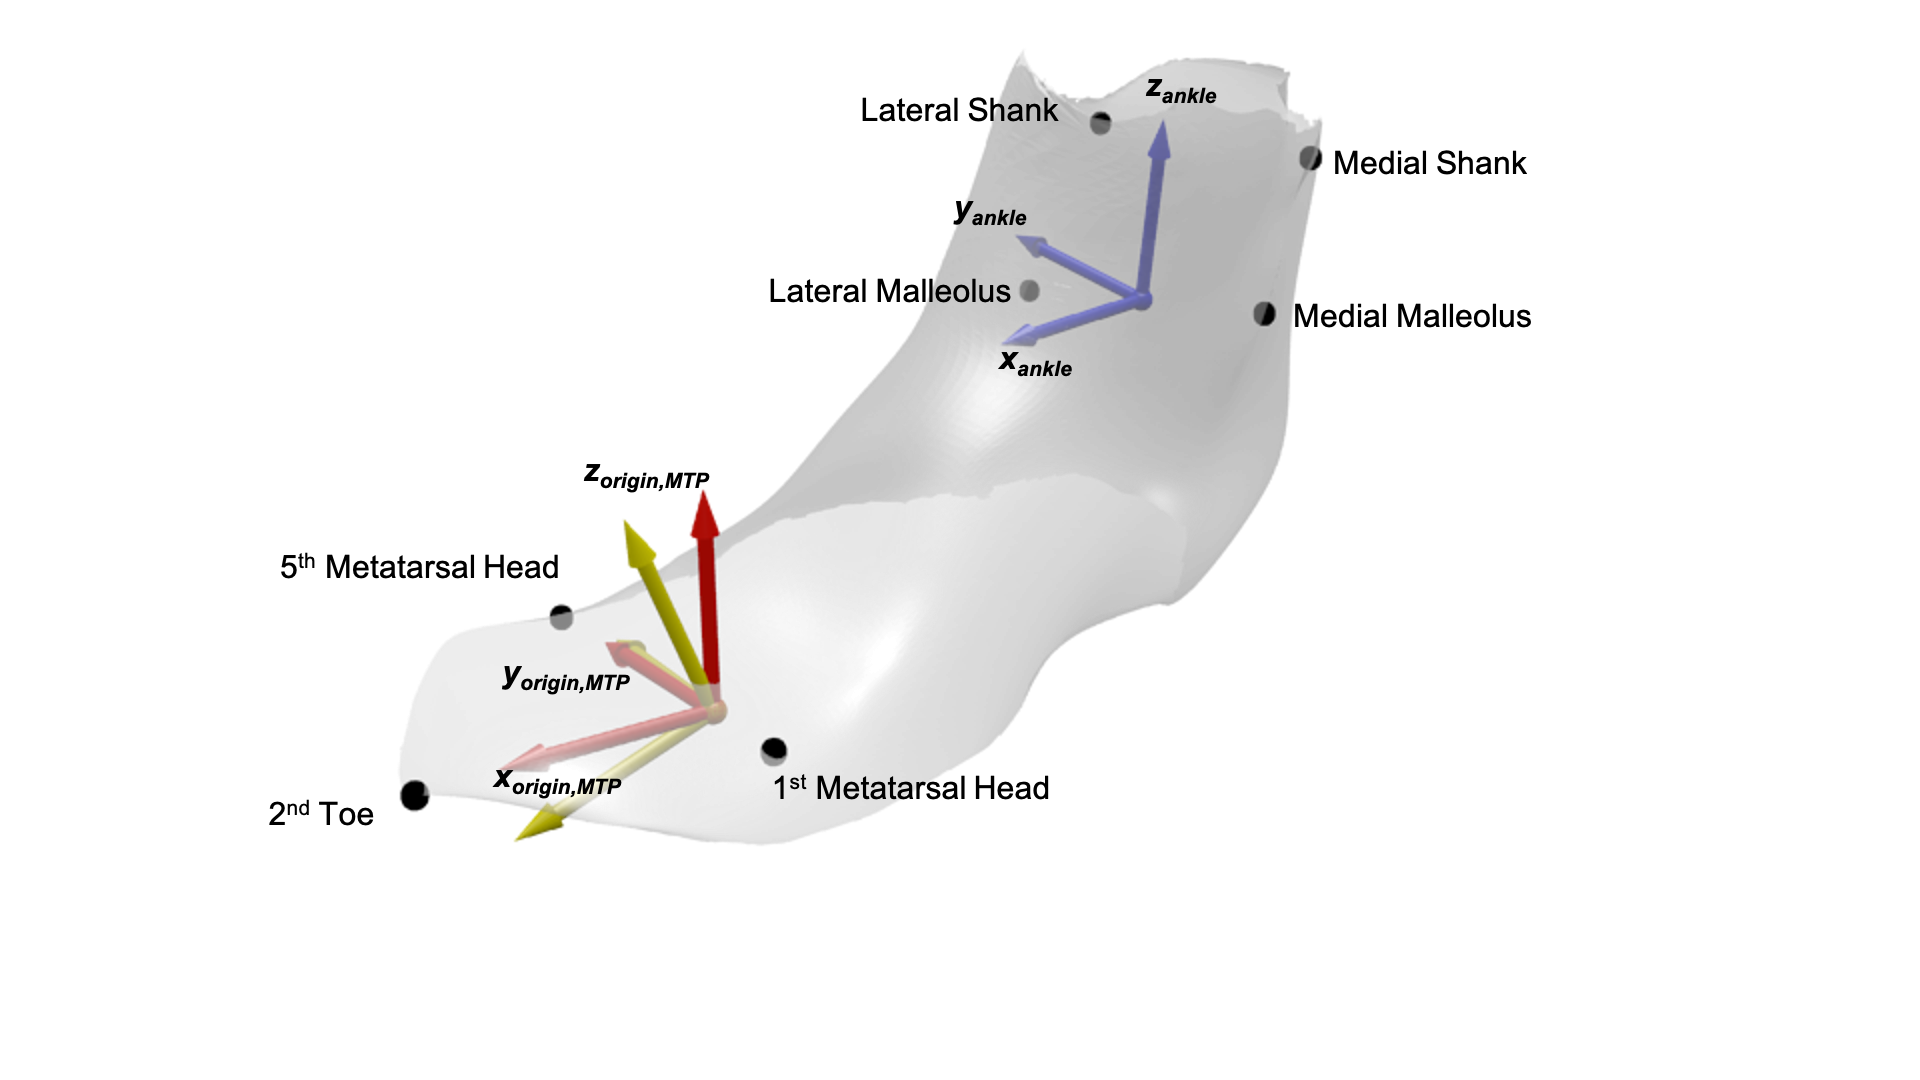
\includegraphics[width=0.9\textwidth,height=\textheight]{fig/coordsystem.png}
\caption{Coordinate system defined from registered scans. Anatomical landmarks are shown as black dots. The ankle joint's local coordinate system is shown in blue, the MTP joint's local coordinate system is shown in yellow, and the model's origin coordinate system is shown in red. Directions for each coordinate system are shown in bold text}\label{fig:supp:angles}
}
\end{figure}
\bibliography{references}
\newpage

\hypertarget{appendix-ii-supplemental-figures}{%
\section*{Appendix II : Supplemental Figures}\label{appendix-ii-supplemental-figures}}
\addcontentsline{toc}{section}{Appendix II : Supplemental Figures}

\begin{figure}
\hypertarget{fig:supp:corr}{%
\centering
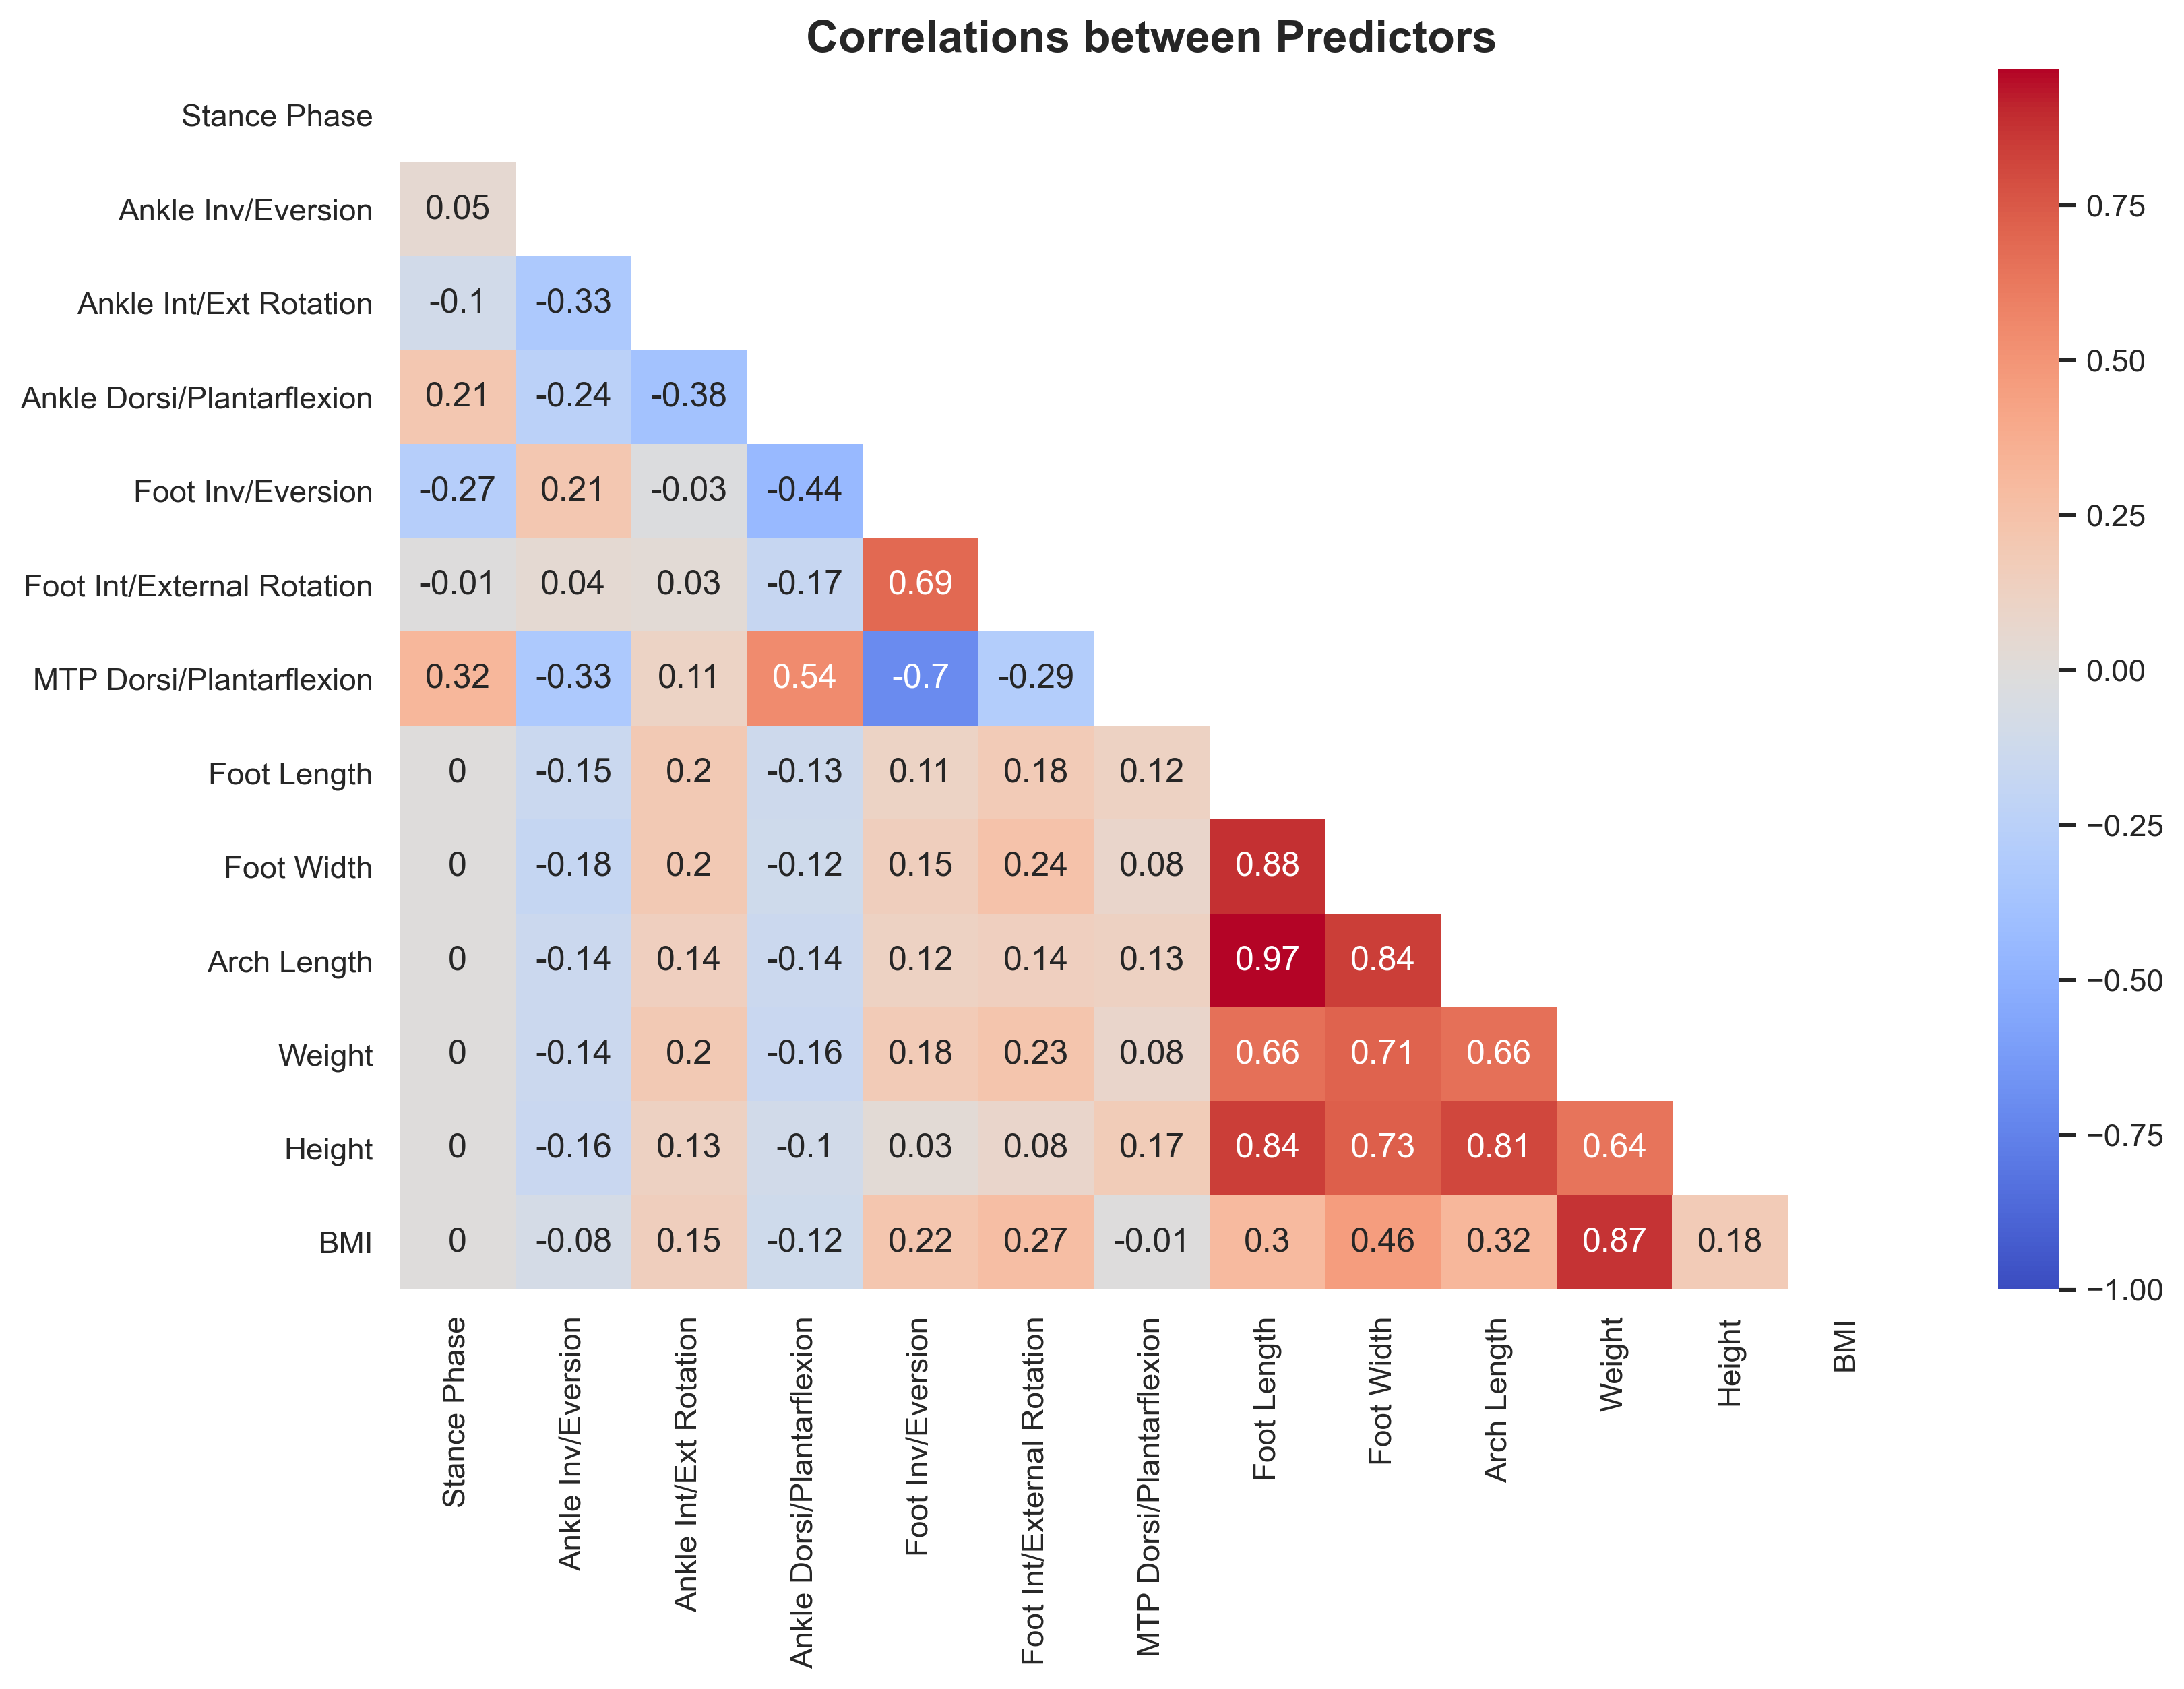
\includegraphics[width=0.9\textwidth,height=\textheight]{fig/supp_corr.png}
\caption{Correlation coefficients across all predictors}\label{fig:supp:corr}
}
\end{figure}

\begin{figure}
\hypertarget{fig:pcav}{%
\centering
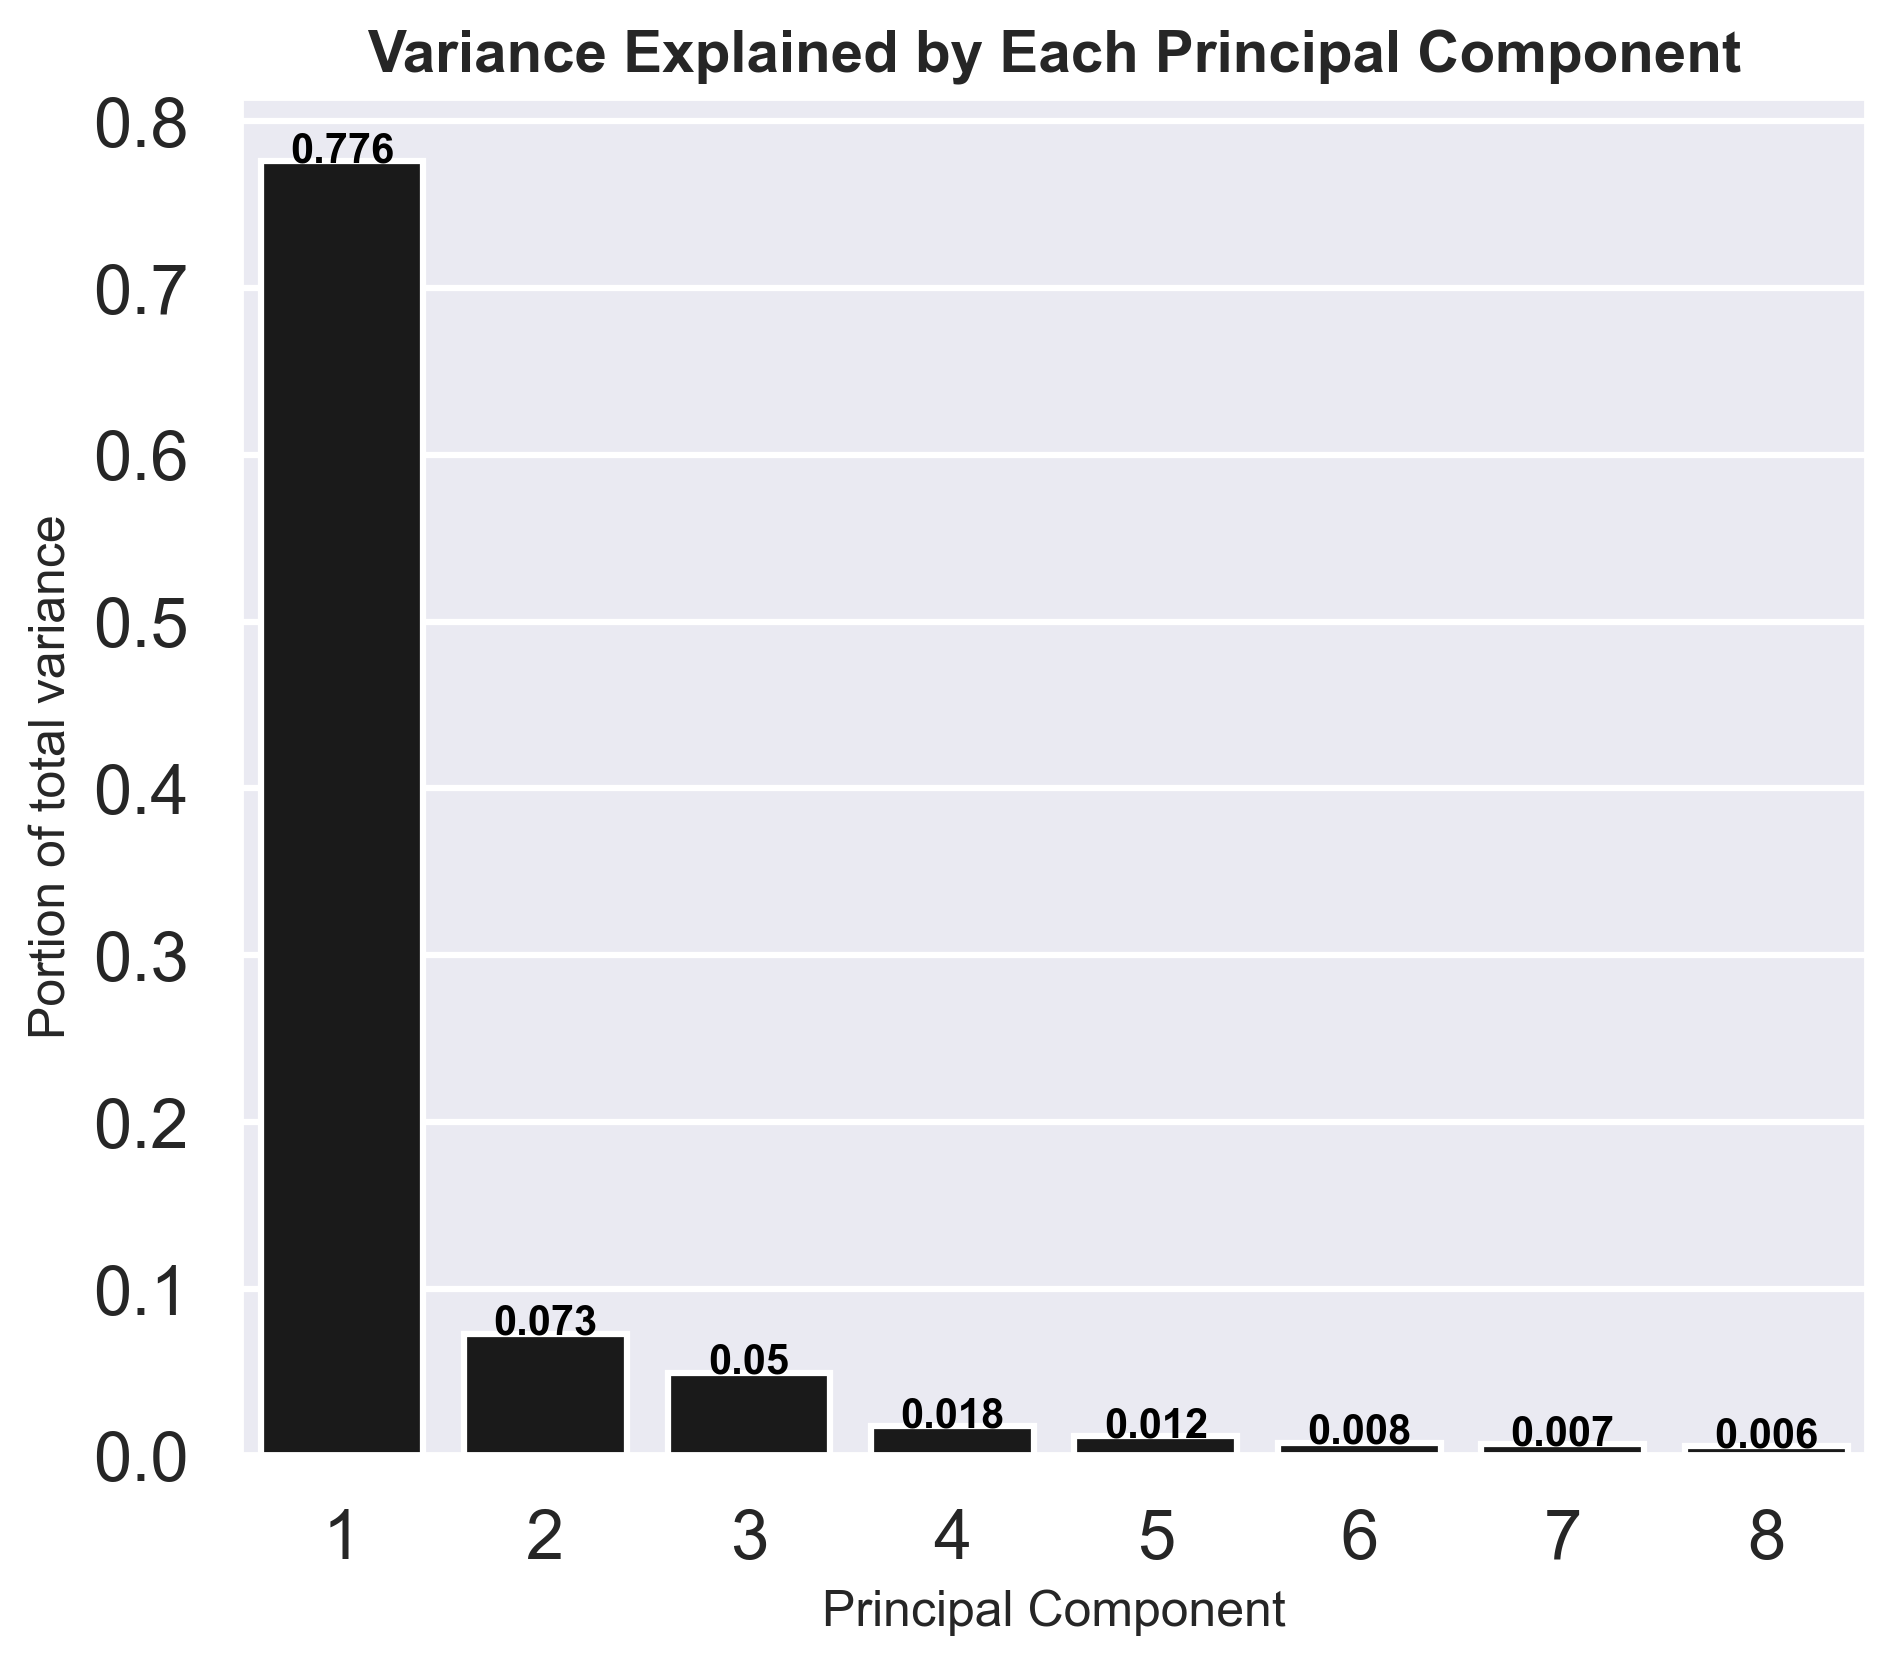
\includegraphics[width=0.7\textwidth,height=\textheight]{fig/PC_variance.png}
\caption{Ratio of total variance explained by each of the first 8 principal components.}\label{fig:pcav}
}
\end{figure}
\newpage
\hypertarget{appendix-iii-supplemental-video}{%
\section*{Appendix III : Supplemental Video}\label{appendix-iii-supplemental-video}}
\addcontentsline{toc}{section}{Appendix III : Supplemental Video}

\url{https://youtu.be/XshzgabhmNE}

The attached video shows the predictive capability of the developed parametric statistical shape model.
The sliders predicts principal component scores, which are then inverse-transformed into a foot shape.
The stance phase slider predicts joint angles during the stance phase to visualize foot morphology changes during stance phase.
% %%\linenumbers

% \section{The Elsevier article class}

% \paragraph{Installation} If the document class \emph{elsarticle} is not available on your computer, you can download and install the system package \emph{texlive-publishers} (Linux) or install the \LaTeX\ package \emph{elsarticle} using the package manager of your \TeX\ installation, which is typically \TeX\ Live or Mik\TeX.

% \paragraph{Usage} Once the package is properly installed, you can use the document class \emph{elsarticle} to create a manuscript. Please make sure that your manuscript follows the guidelines in the Guide for Authors of the relevant journal. It is not necessary to typeset your manuscript in exactly the same way as an article, unless you are submitting to a camera-ready copy (CRC) journal.

% \paragraph{Functionality} The Elsevier article class is based on the standard article class and supports almost all of the functionality of that class. In addition, it features commands and options to format the
% \begin{itemize}
% \item document style
% \item baselineskip
% \item front matter
% \item keywords and MSC codes
% \item theorems, definitions and proofs
% \item lables of enumerations
% \item citation style and labeling.
% \end{itemize}

% \section{Front matter}

% The author names and affiliations could be formatted in two ways:
% \begin{enumerate}[(1)]
% \item Group the authors per affiliation.
% \item Use footnotes to indicate the affiliations.
% \end{enumerate}
% See the front matter of this document for examples. You are recommended to conform your choice to the journal you are submitting to.

% \section{Bibliography styles}

% There are various bibliography styles available. You can select the style of your choice in the preamble of this document. These styles are Elsevier styles based on standard styles like Harvard and Vancouver. Please use Bib\TeX\ to generate your bibliography and include DOIs whenever available.

% Here are two sample references: \cite{Feynman1963118,Dirac1953888}.

% \section*{References}

% \bibliography{mybibfile}

\newpage





\end{document}  